\documentclass{ComputationalAlgorithmsArticle}

\usepackage[dvips]{graphicx}
\usepackage{float}
\usepackage{subfigure}

\usepackage[dvips,
bookmarks,
bookmarksopen,
backref,
colorlinks,linkcolor={blue},citecolor={blue},urlcolor={blue},
]{hyperref}

\title{Morphological Opening on a Graph}

% 
% NOTE: This is the last number of the "handle" URL that 
% The Insight Journal assigns to your paper as part of the
% submission process. Please replace the number "1338" with
% the actual handle number that you get assigned.
%
\newcommand{\IJhandlerIDnumber}{3250}

% Increment the release number whenever significant changes are made.
% The author and/or editor can define 'significant' however they like.
\release{0.00}

% At minimum, give your name and an email address.  You can include a
% snail-mail address if you like.

\author{David Doria}
\authoraddress{Army Research Laboratory, Aberdeen MD}


\begin{document}

\IJhandlefooter{\IJhandlerIDnumber}


\ifpdf
\else
   %
   % Commands for including Graphics when using latex
   % 
   \DeclareGraphicsExtensions{.eps,.jpg,.gif,.tiff,.bmp,.png}
   \DeclareGraphicsRule{.jpg}{eps}{.jpg.bb}{`convert #1 eps:-}
   \DeclareGraphicsRule{.gif}{eps}{.gif.bb}{`convert #1 eps:-}
   \DeclareGraphicsRule{.tiff}{eps}{.tiff.bb}{`convert #1 eps:-}
   \DeclareGraphicsRule{.bmp}{eps}{.bmp.bb}{`convert #1 eps:-}
   \DeclareGraphicsRule{.png}{eps}{.png.bb}{`convert #1 eps:-}
\fi


\maketitle


\ifhtml
\chapter*{Front Matter\label{front}}
\fi

\begin{abstract}
\noindent

This document presents an implementation of an algorithm to perform a morphological opening on a graph. The intent is to remove short branches in a graph while preserving the large scale structure. This implementation is based on the algorithm described in ``Efficient Closed Contour Extraction from Range Image's Edge Points''. We have used the data structures from Boost Graph Library (BGL).

The code is available here:
https://github.com/daviddoria/GraphOpening

\end{abstract}

\IJhandlenote{\IJhandlerIDnumber}

\tableofcontents
%%%%%%%%%%%%%%%%%%%%
\section{Introduction}
This document presents an implementation of an algorithm to perform a morphological opening on a graph. This opening consists of a series of erosions, followed by a series of dilations. This is often done as a first step in contour closure algorithms. This implementation is based on the algorithm described in \cite{Sappa}.

%%%%%%%%%%%%%%%%%%%%
\section{Graph Erosion}
The morphological erosion operation on a graph is defined as removing all edges attached to \emph{end points}. An end point is a vertex with only one incident edge (a vertex with degree 1). The effect of performing multiple iterations of this operation on a graph is that small branches will be "absorbed" into a larger, parent branch.

%%%%%%%%%%%%%%%%%%%%
\section{Graph Dilation}
The morphological dilation operation on a graph is only defined on a graph which has previously been eroded. The dilation adds back edges to current end points that were removed in a previous erosion operation.

%%%%%%%%%%%%%%%%%%%%
\section{Algorithm}
\label{sec:Algorithm}
Now that we have described the two basic operations of erosion and dilation we can describe the morphological opening operation. The algorithm proceeds as follow:
\begin{itemize}
 \item Erode the graph multiple times until a stopping criteria is met
 \item Dilate the graph the same number of times as the graph was eroded
\end{itemize}

Note that this typically does not simply re-grow the original graph. If enough erosions were performed to absorb a branch completely, the branch will not grow back unless the erosion has continued so far that the root of the branch eventually becomes an end point of a future iteration.

\subsection{Stopping Criteria}
\subsubsection{Naive Approach}
The only parameter to be set is how many erosions to perform (as the number of dilations must be the same number).
\subsubsection{Null Removal Difference}
Recall that our goal is to preserve large structure in a graph. A good indication that we have arrived at a ``stable'' large structure is that the number of edges removed in successive erosion operations remains constant for some specified number of iterations. That is, if we remove 3 edges on the first erosion, then 5 edges on the next erosion (a difference of 2), the graph structure is likely still changing. However, if we move 3 edges on the first erosion, then 3 edges on the next erosion (a difference of 0), the graph structure has potentially stabilized, if we proceed with a few more erosions and we continually remove 3 edges, then we can be rather sure that the large scale structure has been found.

\subsection{Speedup}
\subsubsection{Naive Approach}
The most straight forward implementation is to, at each iteration, perform an exhaustive search of the vertices to determine which ones have degree 1. Since finding the end points is the only costly procedure in the algorithm, this is a bad idea.

\subsubsection{Speedup}
An exhaustive search for end points must be performed on the original graph at the beginning of the algorithm. However, at both the erosion and dilation steps, we can search a much smaller set of vertices for end points.
\paragraph{Erosion Speedup}
After each erosion is performed, the set of candidate vertices for the next step (either erosion or dilation) consists of the vertices that were attached to the edges that were removed, excluding the vertices that are now degree 0 (no longer attached to the graph).
\paragraph{Dilation Speedup}
After each dilation, the set of candidate vertices for the next step consists of the vertices that were newly re-attached to the graph.

If an edge was removed in the erosion process, as long as it belonged to the child-most branch that was entirely removed, it will not be regrown in the dilation process.

%%%%%%%%%%%%%%%%%%%%
\section{Demonstration}
\label{sec:Demonstration}
In Figure \ref{fig:1Iteration}, we show the result of one erosion and one dilation. Note that the branches of length 1 were completely removed, while the branch of length 2 was only made shorter.
\begin{figure}[H]
\centering
\subfigure[Original graph.]
  {
  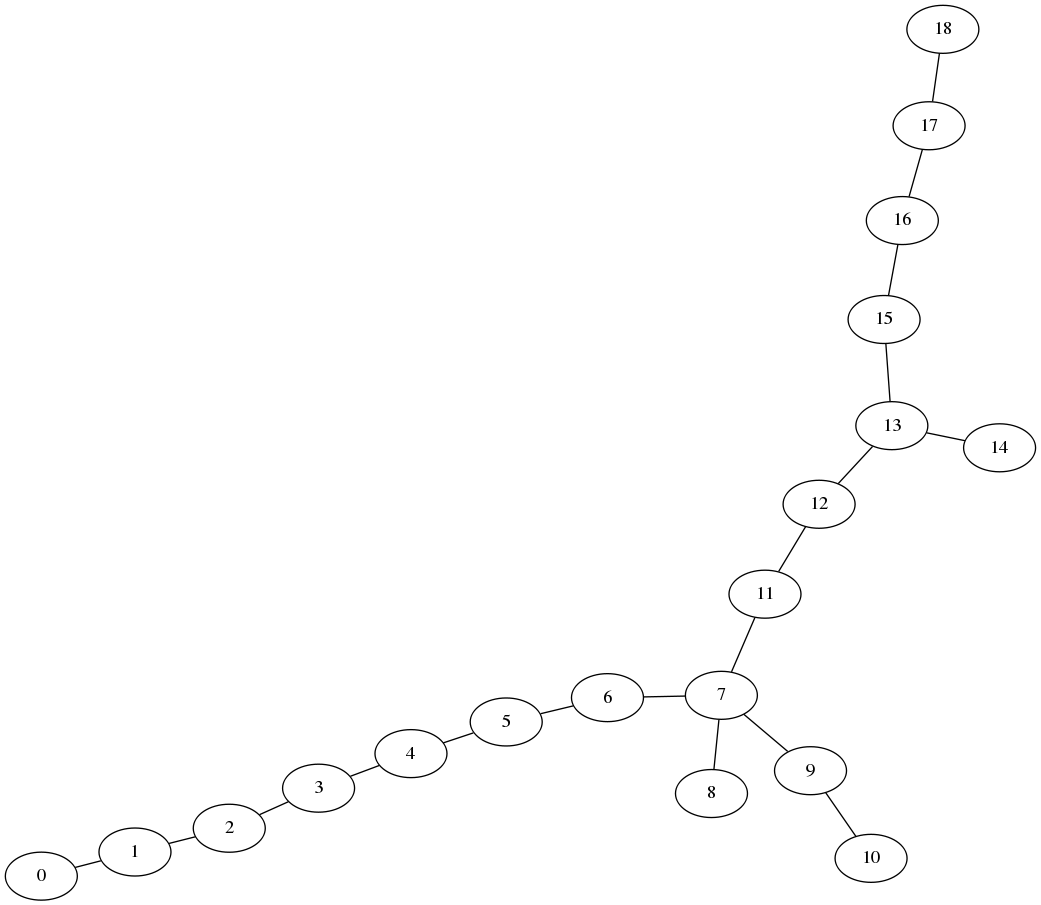
\includegraphics[width=0.3\linewidth]{images/opening1_0}
  \label{fig:1Iteration:Original}
  }
\subfigure[After 1 erosion.]
  {
  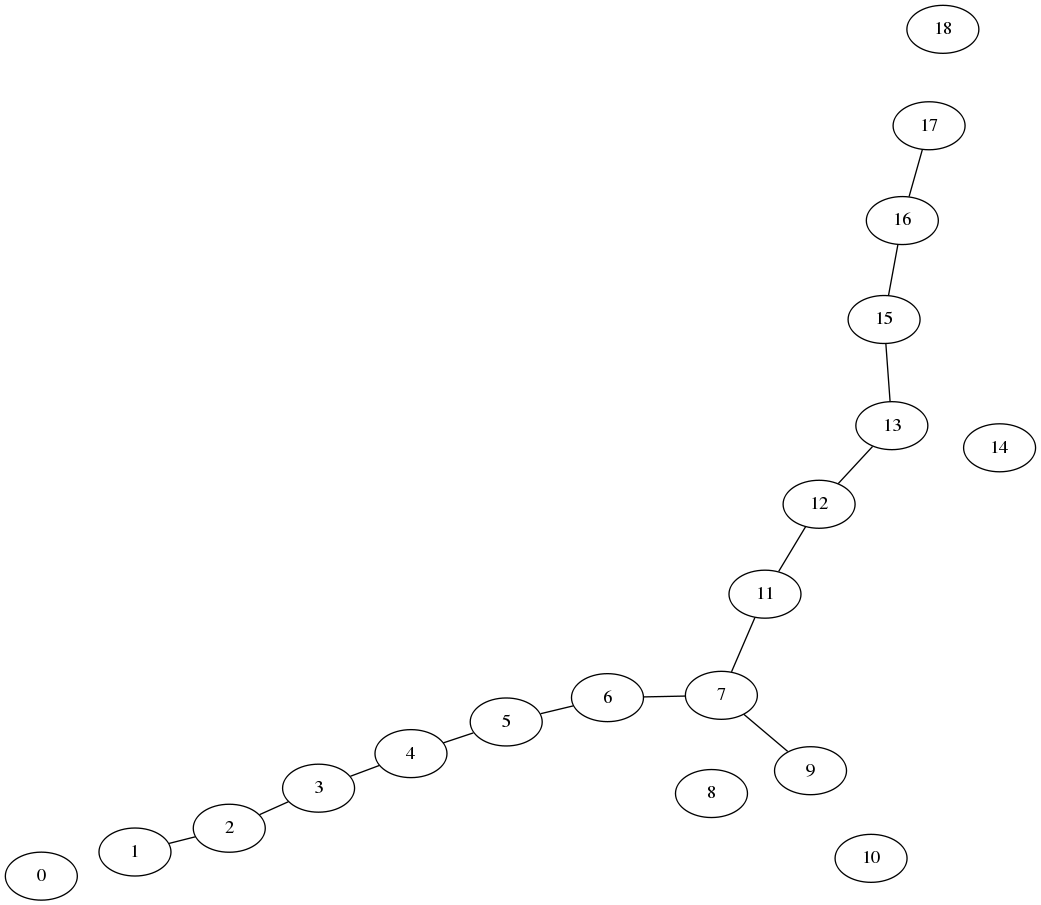
\includegraphics[width=0.3\linewidth]{images/opening1_1}
  \label{fig:1Iteration:1Erosion}
  }
\subfigure[After 1 erosion and 1 dilation.]
  {
  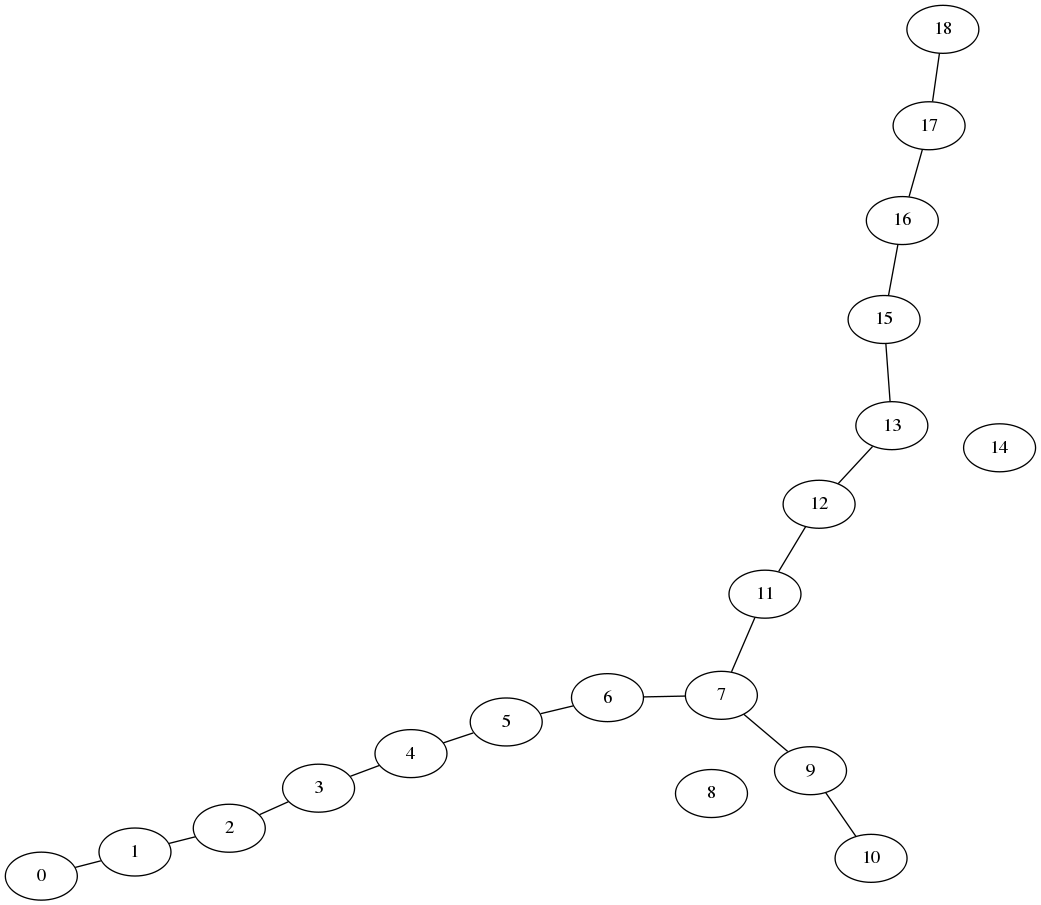
\includegraphics[width=0.3\linewidth]{images/opening1_2}
  \label{fig:1Iteration:1Erosion1Dilation}
  }
\caption{One iteration of the opening operation.}
\label{fig:1Iteration}
\end{figure}

In Figure \ref{fig:2Iterations}, we show the result of one erosion and one dilation. Note that all of the short branches were completely removed, while the large scale structure was preserved. The number of erosions and dilations are indicated in the captions. For example, $\#E=2, \#D=1$ indicates 2 erosions and 1 dilation have been performed.

\begin{figure}[H]
\centering
\subfigure[Original graph.]
  {
  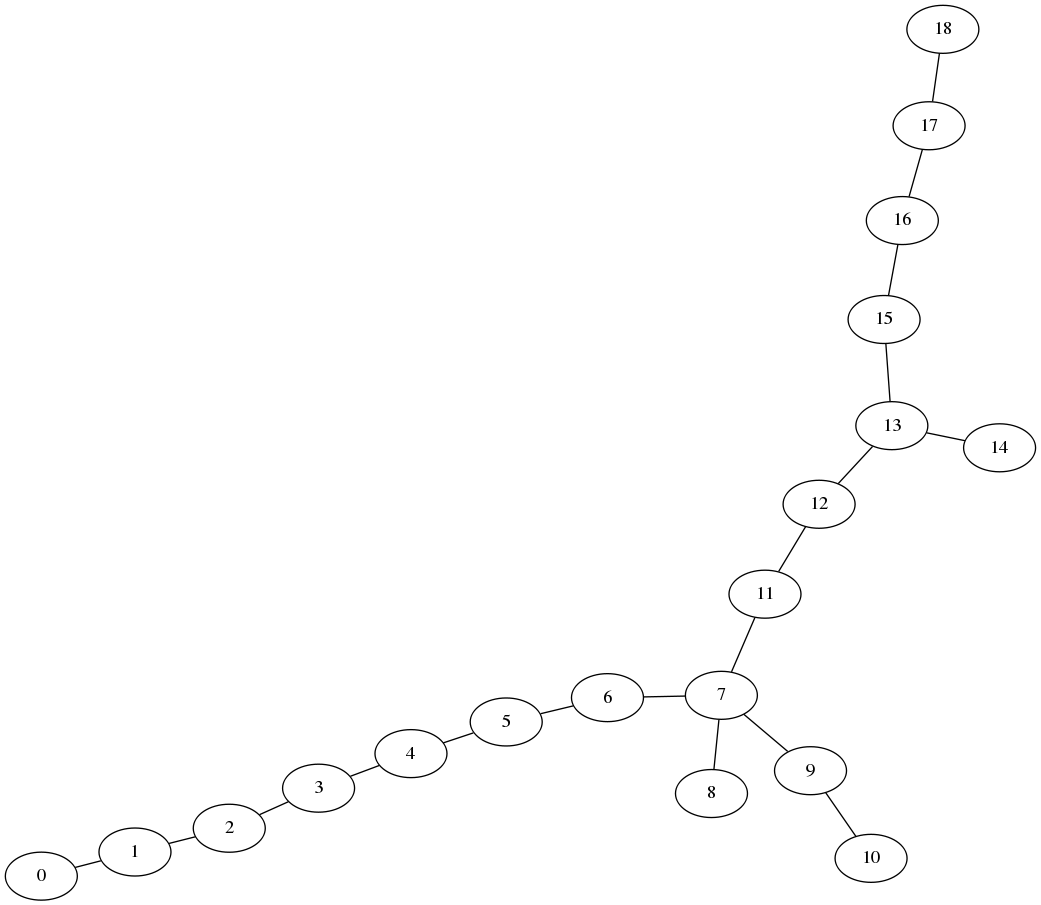
\includegraphics[width=0.17\linewidth]{images/opening2_0}
  \label{fig:2Iterations:Original}
  }
\subfigure[$\#E=1, \#D=0$.]
  {
  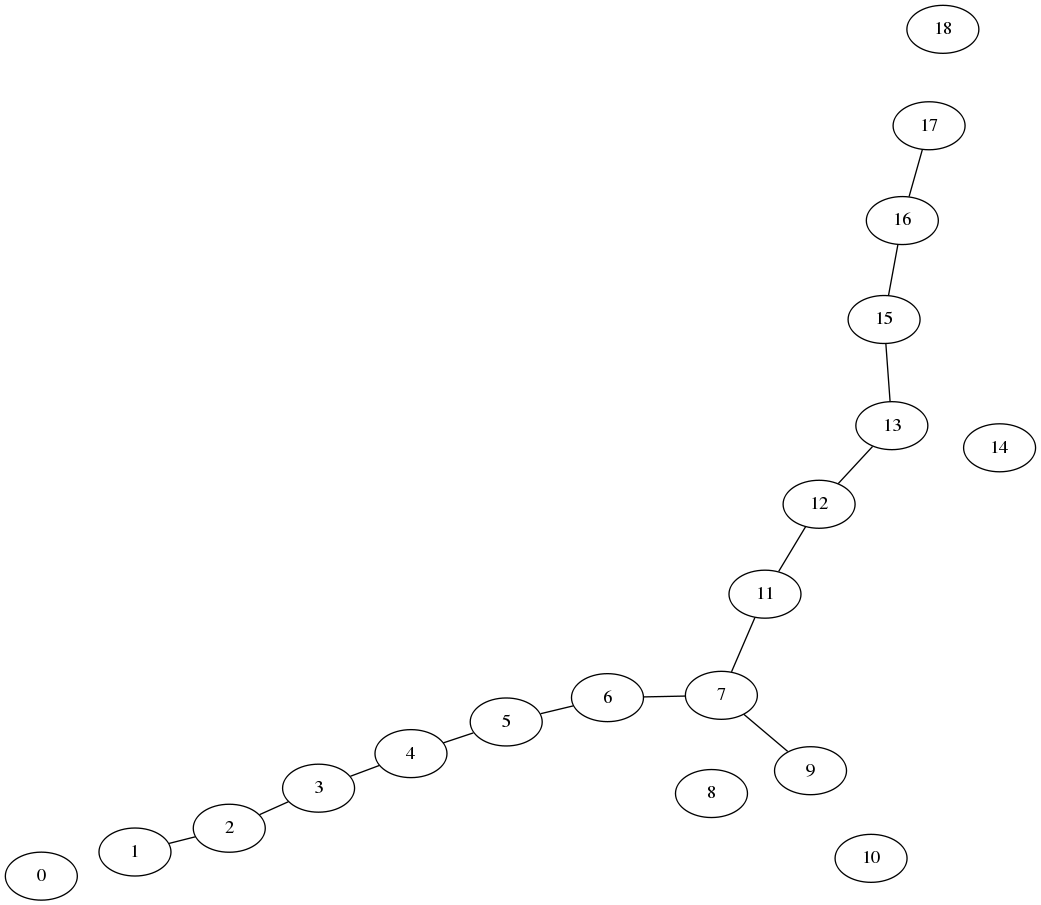
\includegraphics[width=0.17\linewidth]{images/opening2_1}
  \label{fig:2Iterations:1Erosion}
  }
\subfigure[$\#E=2, \#D=0$.]
  {
  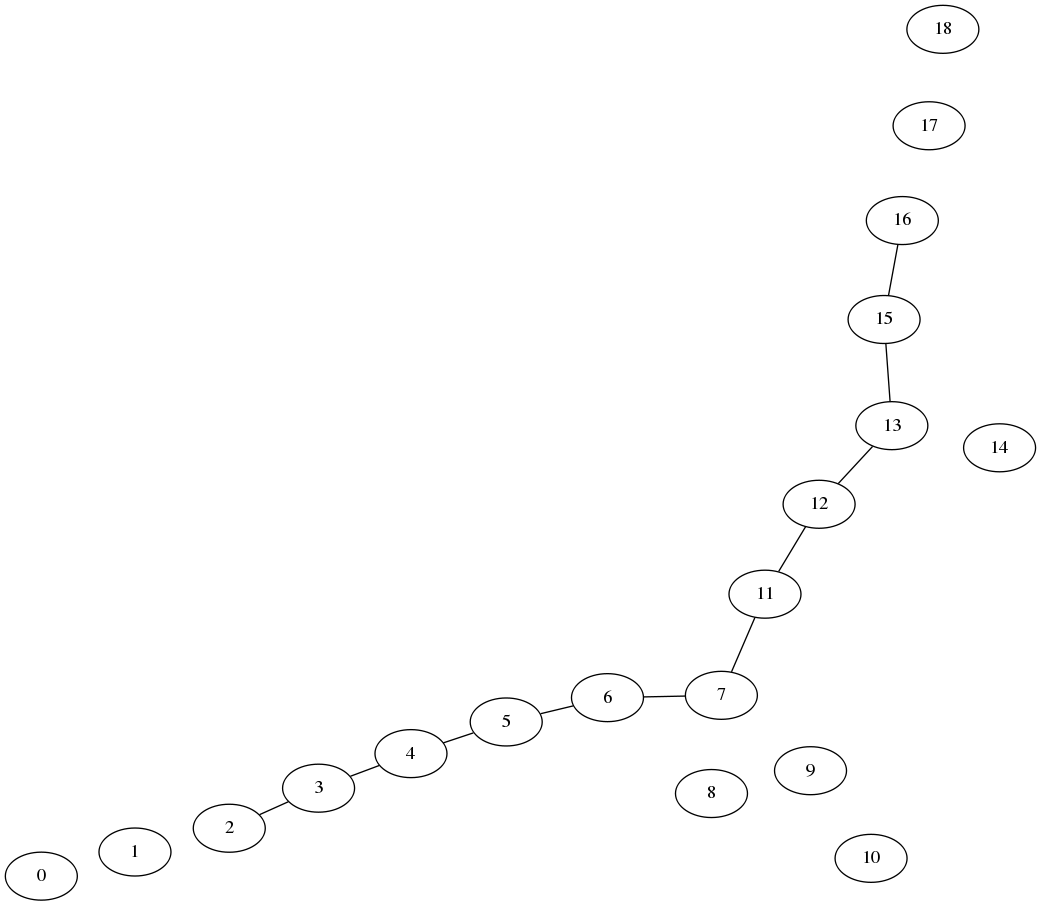
\includegraphics[width=0.17\linewidth]{images/opening2_2}
  \label{fig:2Iterations:2Erosions}
  }
\subfigure[$\#E=2, \#D=1$.]
  {
  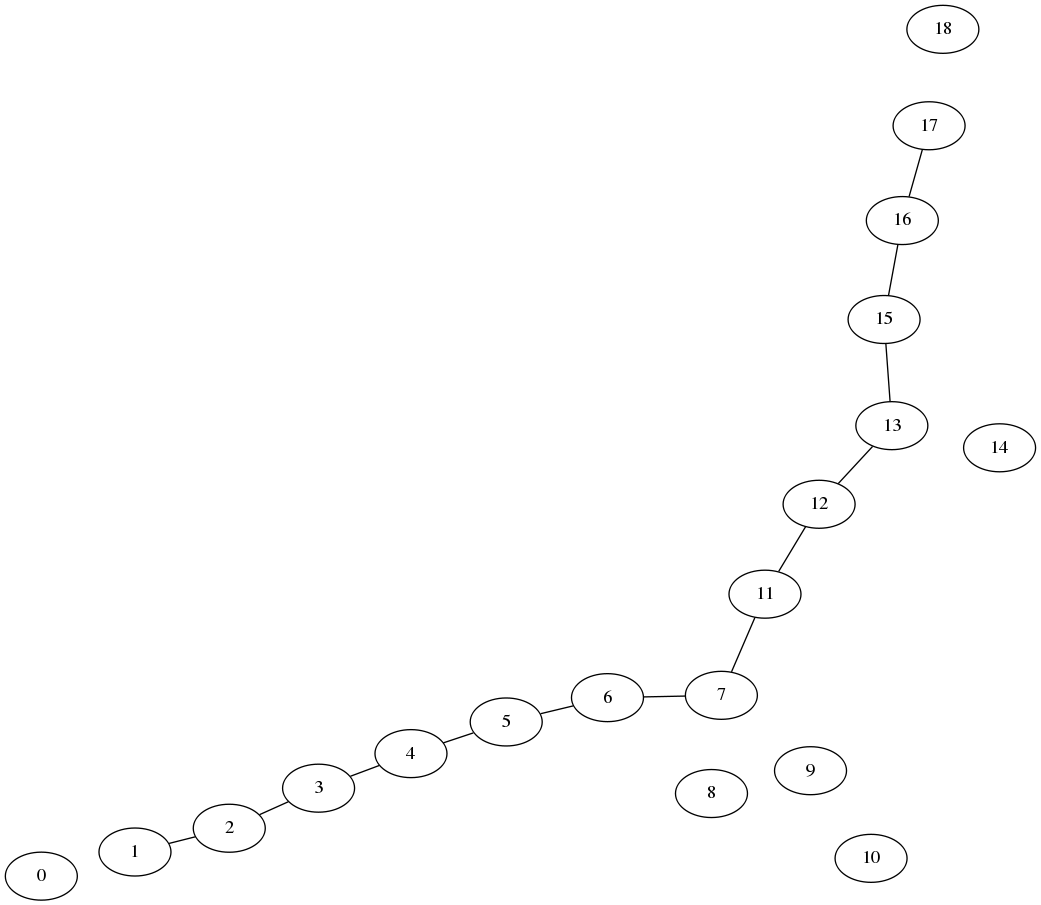
\includegraphics[width=0.17\linewidth]{images/opening2_3}
  \label{fig:2Iterations:2Erosions1Dilation}
  }
\subfigure[$\#E=2, \#D=2$.]
  {
  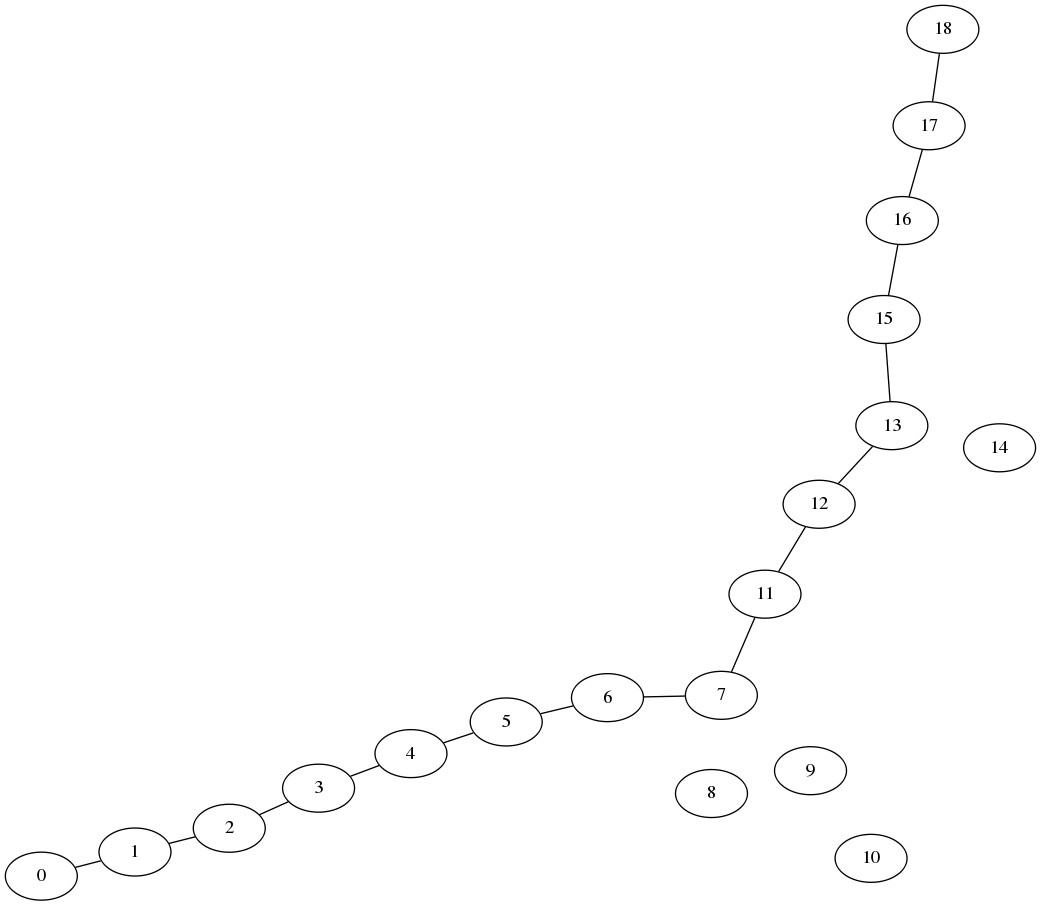
\includegraphics[width=0.17\linewidth]{images/opening2_4}
  \label{fig:2Iterations:2Erosions2Dilations}
  }
\caption{Two iterations of the opening operation.}
\label{fig:2Iterations}
\end{figure}

%%%%%%%%%%%%%%%
\section{Code Breakdown}
\begin{itemize}
 \item Types.h - Defines the graph structure used throughout this code.
 \item Helpers.h/cxx - Defines several functions that are not related to the morphological operations. These are supporting functions for the algorithm implementations.
 \item GraphOpeningNaive.*, GraphOpeningNaiveExample.cxx - This is the naive implementation of the algorithm, where the search for end points is exhaustive.
 \item GraphOpeningTracking.*, GraphOpeningTrackingExample.cxx - This is the implementation of the speedup which tracks potential end points during each operation. You should use these functions in a real application.
 \item GraphOpeningNullRemovalDifferenceExample.cxx - This example demonstrates the successive null edge removal difference stopping crition.
 \item Demo.cxx - There is significant overhead in producing images of graphs with missing edges without the vertices being repositioned. To do this, after each operation we create a graph with identical structure to the original graph, but with edges that have been removed marked as ``invisible''. The layout program ('neato' from 'graphviz'), then positions the vertices identically, but does not draw the edges that should have been removed. This is necessary for easy visualization of each step of the algorithm, but should not be done in a production application.
\end{itemize}

%%%%%%%%%%%%%%%
\section{Code Snippet}
The interface to the code is very simple, as shown below:
\begin{verbatim}
  Graph graph = ReadGraph("input.dot");
  unsigned int numberOfIterations = 2;
  Graph openedGraph = OpenGraphFixedTracking(graph, numberOfIterations);
  WriteGraph(openedGraph, "output.dot");
\end{verbatim}


%%%%%%%%%%%%%%%
\begin{thebibliography}{9}

	\bibitem{Sappa}
	  Sappa, A,
	  \emph{Efficient Closed Contour Extraction from Range Image's Edge Points}.
	  Proceedings of the 2005 IEEE International Conference on Robotics and Automation

\end{thebibliography}

\end{document}